% Options for packages loaded elsewhere
\PassOptionsToPackage{unicode}{hyperref}
\PassOptionsToPackage{hyphens}{url}
\PassOptionsToPackage{dvipsnames,svgnames,x11names}{xcolor}
%
\documentclass[
  letterpaper,
  DIV=11,
  numbers=noendperiod]{scrartcl}

\usepackage{amsmath,amssymb}
\usepackage{iftex}
\ifPDFTeX
  \usepackage[T1]{fontenc}
  \usepackage[utf8]{inputenc}
  \usepackage{textcomp} % provide euro and other symbols
\else % if luatex or xetex
  \usepackage{unicode-math}
  \defaultfontfeatures{Scale=MatchLowercase}
  \defaultfontfeatures[\rmfamily]{Ligatures=TeX,Scale=1}
\fi
\usepackage{lmodern}
\ifPDFTeX\else  
    % xetex/luatex font selection
\fi
% Use upquote if available, for straight quotes in verbatim environments
\IfFileExists{upquote.sty}{\usepackage{upquote}}{}
\IfFileExists{microtype.sty}{% use microtype if available
  \usepackage[]{microtype}
  \UseMicrotypeSet[protrusion]{basicmath} % disable protrusion for tt fonts
}{}
\makeatletter
\@ifundefined{KOMAClassName}{% if non-KOMA class
  \IfFileExists{parskip.sty}{%
    \usepackage{parskip}
  }{% else
    \setlength{\parindent}{0pt}
    \setlength{\parskip}{6pt plus 2pt minus 1pt}}
}{% if KOMA class
  \KOMAoptions{parskip=half}}
\makeatother
\usepackage{xcolor}
\setlength{\emergencystretch}{3em} % prevent overfull lines
\setcounter{secnumdepth}{5}
% Make \paragraph and \subparagraph free-standing
\ifx\paragraph\undefined\else
  \let\oldparagraph\paragraph
  \renewcommand{\paragraph}[1]{\oldparagraph{#1}\mbox{}}
\fi
\ifx\subparagraph\undefined\else
  \let\oldsubparagraph\subparagraph
  \renewcommand{\subparagraph}[1]{\oldsubparagraph{#1}\mbox{}}
\fi


\providecommand{\tightlist}{%
  \setlength{\itemsep}{0pt}\setlength{\parskip}{0pt}}\usepackage{longtable,booktabs,array}
\usepackage{calc} % for calculating minipage widths
% Correct order of tables after \paragraph or \subparagraph
\usepackage{etoolbox}
\makeatletter
\patchcmd\longtable{\par}{\if@noskipsec\mbox{}\fi\par}{}{}
\makeatother
% Allow footnotes in longtable head/foot
\IfFileExists{footnotehyper.sty}{\usepackage{footnotehyper}}{\usepackage{footnote}}
\makesavenoteenv{longtable}
\usepackage{graphicx}
\makeatletter
\def\maxwidth{\ifdim\Gin@nat@width>\linewidth\linewidth\else\Gin@nat@width\fi}
\def\maxheight{\ifdim\Gin@nat@height>\textheight\textheight\else\Gin@nat@height\fi}
\makeatother
% Scale images if necessary, so that they will not overflow the page
% margins by default, and it is still possible to overwrite the defaults
% using explicit options in \includegraphics[width, height, ...]{}
\setkeys{Gin}{width=\maxwidth,height=\maxheight,keepaspectratio}
% Set default figure placement to htbp
\makeatletter
\def\fps@figure{htbp}
\makeatother

\KOMAoption{captions}{tableheading}
\makeatletter
\makeatother
\makeatletter
\makeatother
\makeatletter
\@ifpackageloaded{caption}{}{\usepackage{caption}}
\AtBeginDocument{%
\ifdefined\contentsname
  \renewcommand*\contentsname{Table of contents}
\else
  \newcommand\contentsname{Table of contents}
\fi
\ifdefined\listfigurename
  \renewcommand*\listfigurename{List of Figures}
\else
  \newcommand\listfigurename{List of Figures}
\fi
\ifdefined\listtablename
  \renewcommand*\listtablename{List of Tables}
\else
  \newcommand\listtablename{List of Tables}
\fi
\ifdefined\figurename
  \renewcommand*\figurename{Figure}
\else
  \newcommand\figurename{Figure}
\fi
\ifdefined\tablename
  \renewcommand*\tablename{Table}
\else
  \newcommand\tablename{Table}
\fi
}
\@ifpackageloaded{float}{}{\usepackage{float}}
\floatstyle{ruled}
\@ifundefined{c@chapter}{\newfloat{codelisting}{h}{lop}}{\newfloat{codelisting}{h}{lop}[chapter]}
\floatname{codelisting}{Listing}
\newcommand*\listoflistings{\listof{codelisting}{List of Listings}}
\makeatother
\makeatletter
\@ifpackageloaded{caption}{}{\usepackage{caption}}
\@ifpackageloaded{subcaption}{}{\usepackage{subcaption}}
\makeatother
\makeatletter
\@ifpackageloaded{tcolorbox}{}{\usepackage[skins,breakable]{tcolorbox}}
\makeatother
\makeatletter
\@ifundefined{shadecolor}{\definecolor{shadecolor}{rgb}{.97, .97, .97}}
\makeatother
\makeatletter
\makeatother
\makeatletter
\makeatother
\ifLuaTeX
  \usepackage{selnolig}  % disable illegal ligatures
\fi
\IfFileExists{bookmark.sty}{\usepackage{bookmark}}{\usepackage{hyperref}}
\IfFileExists{xurl.sty}{\usepackage{xurl}}{} % add URL line breaks if available
\urlstyle{same} % disable monospaced font for URLs
\hypersetup{
  pdftitle={Data Wells: Race and State Violence in the United States from 1892},
  pdfauthor={Nathan Alexander; Kade Davis; Basil Ghali; Qyana Stewart; Gabriella La Cour},
  colorlinks=true,
  linkcolor={blue},
  filecolor={Maroon},
  citecolor={Blue},
  urlcolor={Blue},
  pdfcreator={LaTeX via pandoc}}

\title{Data Wells: Race and State Violence in the United States from
1892}
\usepackage{etoolbox}
\makeatletter
\providecommand{\subtitle}[1]{% add subtitle to \maketitle
  \apptocmd{\@title}{\par {\large #1 \par}}{}{}
}
\makeatother
\subtitle{Quantitative Histories Workshop}
\author{Nathan Alexander \and Kade Davis \and Basil Ghali \and Qyana
Stewart \and Gabriella La Cour}
\date{}

\begin{document}
\maketitle
\ifdefined\Shaded\renewenvironment{Shaded}{\begin{tcolorbox}[sharp corners, boxrule=0pt, frame hidden, interior hidden, breakable, enhanced, borderline west={3pt}{0pt}{shadecolor}]}{\end{tcolorbox}}\fi

\renewcommand*\contentsname{Table of contents}
{
\hypersetup{linkcolor=}
\setcounter{tocdepth}{3}
\tableofcontents
}
\hypertarget{data-ida-b.-wells-barnett}{%
\subsection{\texorpdfstring{{\emph{Data}} + Ida B.
{\emph{Wells}}-Barnett}{Data + Ida B. Wells-Barnett}}\label{data-ida-b.-wells-barnett}}

\begin{itemize}
\item
  We use the term ``{Data Wells}'' to describe how we practice the
  identification, input, and storage of what can be termed as critical
  insights data, or CIDs.
\item
  We use information in databases in four ways:

  \begin{enumerate}
  \def\labelenumi{(\arabic{enumi})}
  \item
    studying problems in the {quantification of historical information}
    across various axes: time, social constructs, and/or systemic
    issues,
  \item
    data {identification} and {wrangling},
  \item
    data {analysis} and {communication}, and
  \item
    {modeling} abstract inquiries.
  \end{enumerate}
\item
  We begin our analysis with Ida B. Wells-Barnett's organization and
  analysis of lynching.
\item
  We describe ``Data Wells'' of U.S. state violence using quantitative
  history as a frame.
\end{itemize}

\hypertarget{quantitative-histories-workshop}{%
\section{Quantitative Histories
Workshop}\label{quantitative-histories-workshop}}

\texttt{Curriculum\ \&\ software\ development\ collective}

and

{research lab}

\hypertarget{quantitative-history}{%
\subsection{Quantitative history}\label{quantitative-history}}

\begin{itemize}
\item
  Quantitative history considers methods and approaches to artifacts as
  data and information.
\item
  Historians like Pierre Chanu (text to right) are centered in
  traditional texts; more perspectives are uncovering troubling
  practices with regard to race\footnote{Vovelle, Michel (1987).
    Bourgeoisies de province et Revolution. Presses Universitaires de
    Grenoble.}.
\item
  Despite long-standing critiques, there are {few critical dimensions}
  in \protect\hyperlink{quantitative-history}{quantitative history}
  narratives.
\end{itemize}

\begin{figure}

{\centering 
\includegraphics[width=0.4\textwidth,height=\textheight]{quanthist.jpg}

}

\caption{\href{https://www.jstor.org/stable/1876930}{\emph{Histoire
Quantitative}} by Pierre Chanu}

\end{figure}

\hypertarget{racialization-and-u.s.-state-violence}{%
\subsection{Racialization and U.S. State
Violence}\label{racialization-and-u.s.-state-violence}}

Today, we will discuss race and racialization in \emph{data wells} of
state sponsored violence:

. . .

\begin{itemize}
\tightlist
\item
  Lynching
\end{itemize}

. . .

\begin{itemize}
\tightlist
\item
  Policing
\end{itemize}

. . .

\begin{itemize}
\tightlist
\item
  Prisons
\end{itemize}

\hypertarget{ida-b.-wells-barnett-on-lynching}{%
\subsection{Ida B. Wells-Barnett on
lynching}\label{ida-b.-wells-barnett-on-lynching}}

\begin{itemize}
\tightlist
\item
  \textbf{Personal experience}. In 1892, a close friend of Ida B.
  Wells-Barnett was lynched. Wells-Barnett, a known activist, community
  organizer, and journalist, would generate quantitative indicators of
  lynching as state violence.
\end{itemize}

. . .

\begin{itemize}
\tightlist
\item
  \textbf{Intuition and method}. Like many Black communities at the time
  and other allies, Wells-Barnett acknowledged both the personal (micro)
  social forces of racism and the systemic (macro) nature of white
  racial violence. In this case, this violence was expressed through the
  practice of lynching.
\end{itemize}

. . .

\begin{itemize}
\tightlist
\item
  \textbf{Impact}. Wells-Barnett's databases, and the use of number and
  quantification have a profound impact on the current view of
  state-sponsored racial violence.
\end{itemize}

\hypertarget{lynching}{%
\subsection{Lynching}\label{lynching}}

Caitlin Pollock has created
\href{https://redrecord.cmjpollock.com/}{software} based on a series of
extracted data from Wells-Barnett's work. Although the data provides for
quick loading and analysis, it does require some data wrangling.

\subsubsection{1893}

Content for 1893

\subsubsection{1893 map}

\subsubsection{1894}

Content for 1894

\subsubsection{1895}

Content for 1895

\begin{center}\rule{0.5\linewidth}{0.5pt}\end{center}

\hypertarget{concerns}{%
\subsection{Concerns}\label{concerns}}

Pollock deals with the issue of erasure in their development of the
data.

\hypertarget{policing}{%
\subsection{Policing}\label{policing}}

\hypertarget{fatal-police-interactions}{%
\subsection{Fatal police interactions}\label{fatal-police-interactions}}

\begin{figure}

{\centering 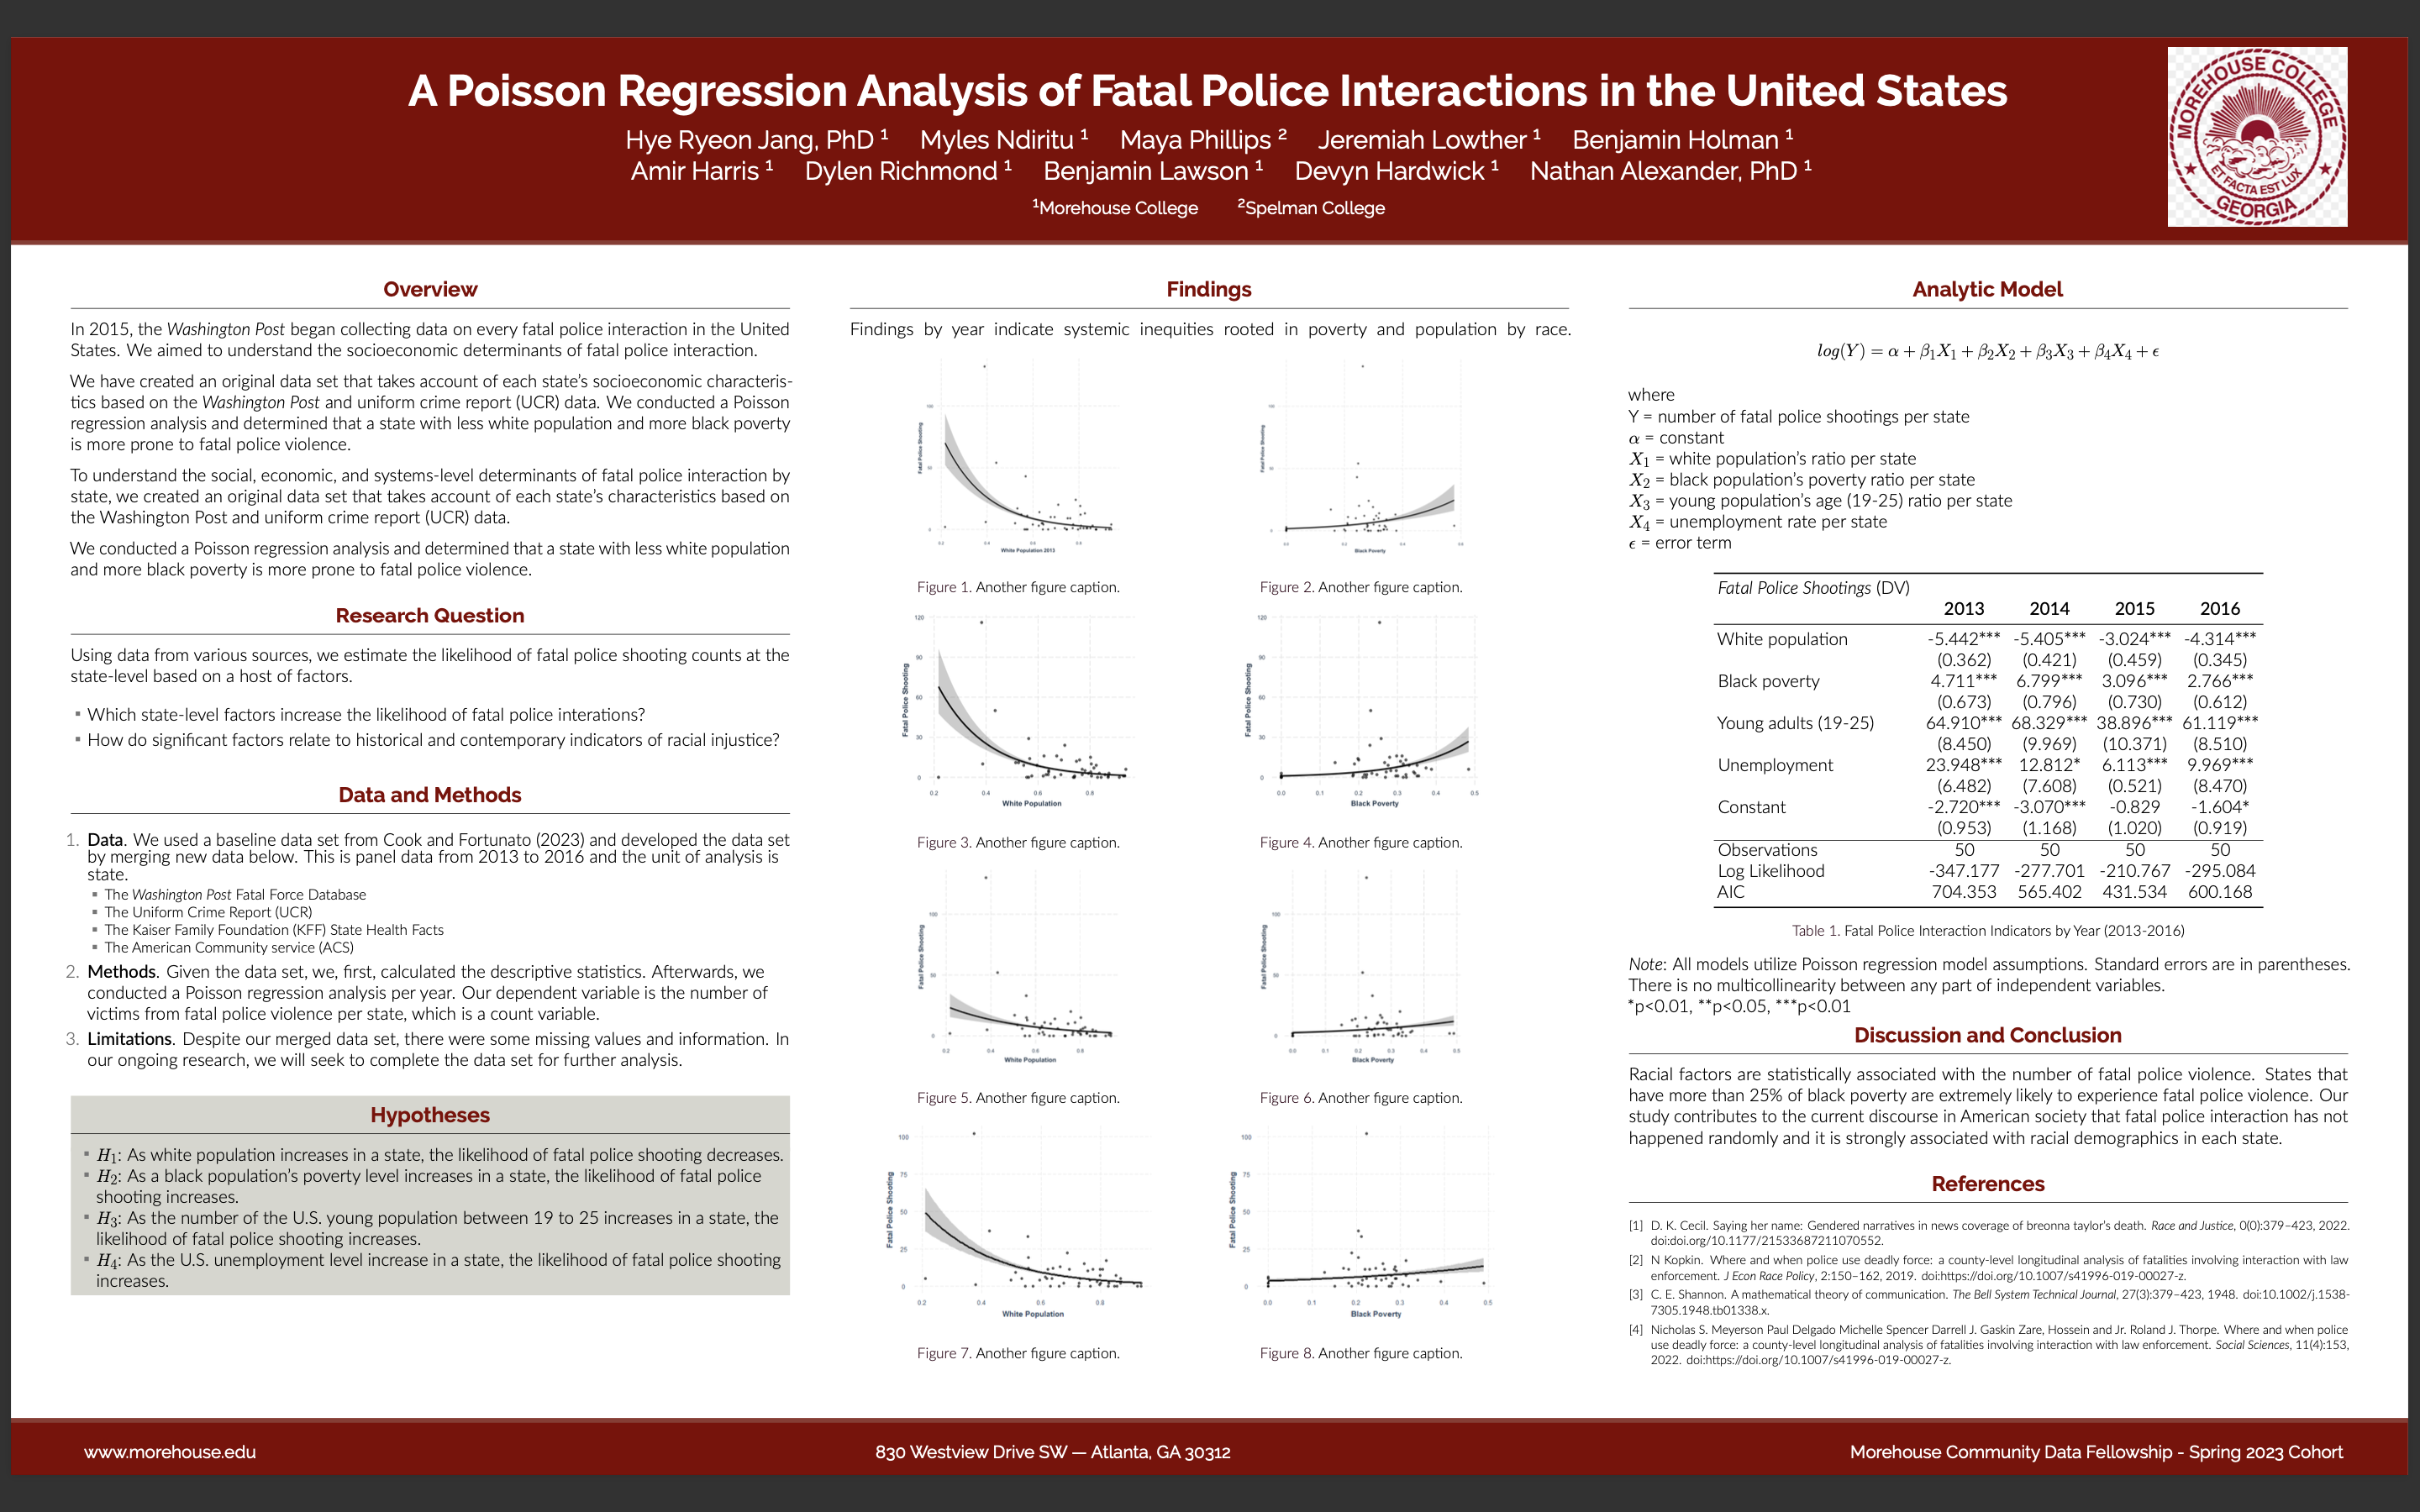
\includegraphics{poster3.png}

}

\caption{Faculty and student research poster}

\end{figure}

\hypertarget{campus-policing}{%
\subsection{Campus Policing}\label{campus-policing}}

\hypertarget{campus-policing-timeline}{%
\subsection{Campus Policing Timeline}\label{campus-policing-timeline}}

\hypertarget{racism}{%
\subsection{Racism}\label{racism}}

\hypertarget{prisons}{%
\subsection{Prisons}\label{prisons}}

\begin{itemize}
\item
  ``In 2021, Black Americans were imprisoned at 5.0 times the rate of
  whites, while American Indians and Latinx people were imprisoned at
  4.2 times and 2.4 times the white rate, respectively.''
  (\href{https://www.sentencingproject.org/reports/one-in-five-ending-racial-inequity-in-incarceration/}{The
  Sentencing Project}, 2023)
\item
  ``One in five Black men born in 2001 is likely to experience
  imprisonment within their lifetime, a decline from one in three for
  those born in 1981. Pushback from policymakers threatens further
  progress in reducing racial inequity in incarceration.''
  (\href{https://www.sentencingproject.org/reports/one-in-five-ending-racial-inequity-in-incarceration/}{The
  Sentencing Project}, 2023)
\end{itemize}

\hypertarget{prisons-1}{%
\subsection{Prisons}\label{prisons-1}}

The U.S. Bureua of Justice Statistics maintains records of federal and
state prison populations\footnote{Source of data:
  \href{https://bjs.ojp.gov/library/publications/prisoners-2021-statistical-tables}{Carson
  (2022). Prisoners in 2021 -- Statistical tables. Bureau of Justice
  Statistics.}}.

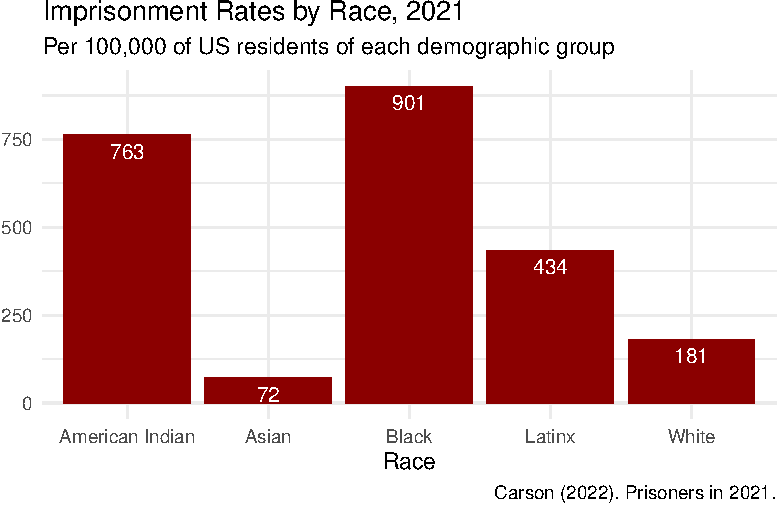
\includegraphics{2024_04_27_bob_moses_files/figure-pdf/unnamed-chunk-9-1.pdf}

\hypertarget{prisons-2}{%
\subsection{Prisons}\label{prisons-2}}

\subsubsection{Federal}

Content for federal

\subsubsection{State}

Content for state

\subsubsection{Federal and State}

Content for federal and state

\hypertarget{thank-you}{%
\section{Thank you}\label{thank-you}}

. . .

Thank you for joining us and citing today's presentation.

Alexander, N., Davis, K., Ghali, B., Stewart, K., \& La Cour, G. (2024,
April 26). Data Wells: Race and State Violence in the United States from
1892. \emph{The 2024 Bob Moses Conference}.
\href{https://www.bobmosesconference.com/}{Online}.



\end{document}
